\documentclass[aspectratio=169]{beamer}
\usepackage[utf8]{inputenc}
\usepackage{minted}
\usepackage{listings}
\usetheme{veit}
\title{All I have is a hammer, now give me your nails!}
\date{\today}
\author{Veit Heller}
\institute{EnthusiastiCon 2020}
\begin{document}
  \maketitle
  \begin{frame}{Motivation}
    “If all you have is a hammer, everything looks like a nail.” -- Every
    programmer ever
  \end{frame}
  \begin{frame}{Motivation}
    But: is it always bad to see the world through a particular lens?
  \end{frame}
  \begin{frame}{Motivation}
    “It is better to have 100 functions operate on one data structure than 10
    functions on 10 data structures.” -- Alan Perlis
  \end{frame}
  \begin{frame}{Motivation}
    What do you get if you try to make everything one data structure?
  \end{frame}
  \section{Lisp}
  \begin{frame}[fragile]
    \frametitle{Lisp}
    \begin{listing}[H]
      \caption{A definition of \texttt{and}.}
      \begin{minted}{clojure}
(defmacro and [:rest args]
  (list 'if (first args) (list 'and (rest args)) false))
      \end{minted}
    \end{listing}
  \end{frame}
  \section{SmallTalk}
  \begin{frame}[fragile]
    \frametitle{SmallTalk}
    \begin{listing}[H]
      \caption{Booleans as objects.}
      \begin{minted}{smalltalk}
True >> ifTrue: trueBlock ifFalse: falseBlock [
  ^ trueBlock value
]

False >> ifTrue: trueBlock ifFalse: falseBlock [
  ^ falseBlock value
]
      \end{minted}
    \end{listing}
  \end{frame}
  \section{Forth}
  \begin{frame}[fragile]
    \frametitle{Forth}
    \begin{listing}[H]
      \caption{Comments on the stack.}
      \begin{minted}{forth}
: ( 41 WORD DROP ; IMMEDIATE
      \end{minted}
    \end{listing}
  \end{frame}
  \section{APL}
  \begin{frame}{APL}
    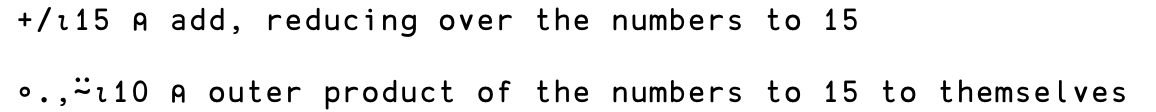
\includegraphics[width=12cm]{apl}
  \end{frame}
  \section{So what?}
  \begin{frame}{Conclusion?}
    This is neat, but what is the appeal, really?

    What do we gain?
  \end{frame}
  \begin{frame}{Conclusion}
    Basing all of your thinking on one axiom answers a lot of questions.
  \end{frame}
  \begin{frame}{Conclusion}
    It also asks a lot of questions.
  \end{frame}
  \begin{frame}{Conclusion}
    Beyond pure novelty, there is a liberating quality to seeing the world
    through a particular lens.

    Constraints can be liberating!
  \end{frame}
  \begin{frame}{}
    Thank you!
  \end{frame}
\end{document}
